% Distance-based evaluation of the generated sequences (definitions in section sec:distances).
% Numbers from evaluations/<run>/metrics.json ["distances"].

\section{Results: distances between generated and real sequences}\label{sec:res_dist}
All quantities are defined in \S\ref{sec:distances}. They were computed for the four trained models; this
section reports the two $H=128$ models, and the $H=256$ models are compared in \S\ref{sec:res_H256}.

\subsection{Novelty: distance to the nearest training sequence}
\begin{center}\small
\begin{tabular}{lcccc}
\toprule
 & mean $d_{NN}$ & copies of a & $W_1$ vs & mean $d_{NN}$\\
 & to train & train seq. & test & of test seqs\\
\midrule
oracle (fresh true samples) & 0.378 & 0\% & 0.001 & 0.378\\
unconditioned, $H=128$ & 0.398 & 0\% & 0.019 & 0.378\\
conditioned, $H=128$ (per clade, mean) & 0.370 & 0\% & 0.011 & 0.378\\
\bottomrule
\end{tabular}
\end{center}
\textbf{No model copies its training data.} Not one of the 36{,}000 generated sequences equals a training sequence.
A typical held-out real sequence differs from its closest training sequence at 37.8\% of its sites
($\approx23$ of 60). The generated sequences are about as novel: the conditioned model's are marginally
\emph{closer} to the training set (0.370, i.e.\ half a site less), consistent with their slight over-conservation.
The unconditioned model's are slightly \emph{farther} (0.398). Our interpretation: a single Potts model fitted
to the mixture produces some hybrid sequences that combine features of different clades, and such sequences are
far from every training sequence.

\begin{figure}[H]
\centering
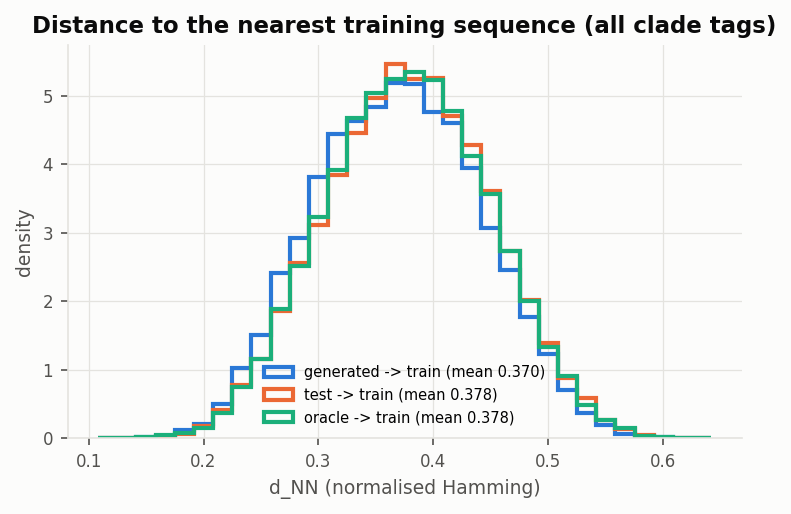
\includegraphics[width=0.49\linewidth]{models/fa_conditional_H128/dist_nn_to_train.png}\hfill
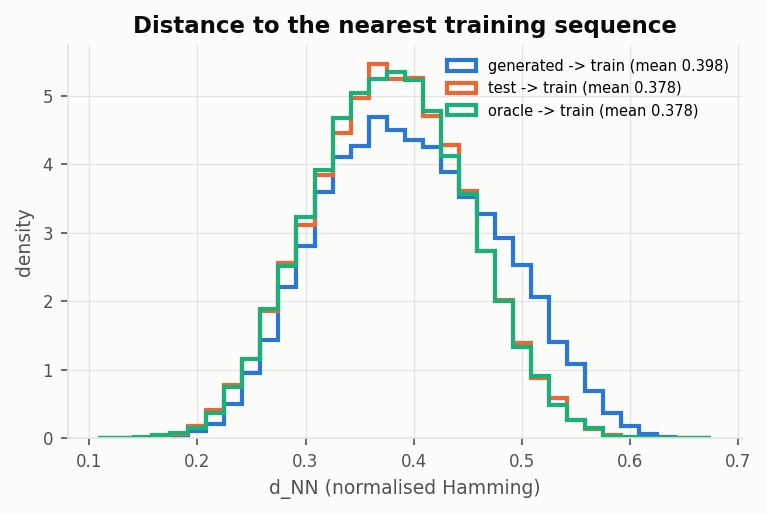
\includegraphics[width=0.49\linewidth]{models/fa_unconditional_H128/dist_nn_to_train.png}
\caption{Distribution of $d_{NN}$ to the training set. Left: conditioned model, all 18 clade tags. Right:
unconditioned model. Generated (blue), held-out test (orange), oracle (green). The oracle and test curves coincide
(same distribution); the generated curve of the conditioned model is shifted left by $\approx0.01$.}
\end{figure}

\subsection{Diversity: pairwise Hamming distances}
\begin{center}\footnotesize
\begin{tabular}{lccccc}
\toprule
 & $\bar D_{GG}$ & $\bar D_{RR}$ & $\bar D_{GR}$ & $W_1(D_{GG},D_{RR})$ & $W_1(D_{GR},D_{RR})$\\
 & (generated) & (test) & & &\\
\midrule
oracle, per clade (mean) & 0.664 & 0.663 & 0.664 & 0.003 & 0.002\\
conditioned $H=128$, per clade (mean) & 0.637 & 0.663 & 0.660 & 0.027 & 0.007\\
\midrule
oracle, pooled & 0.803 & 0.803 & 0.803 & 0.001 & 0.001\\
unconditioned $H=128$, pooled & 0.740 & 0.803 & 0.786 & 0.063 & 0.018\\
\bottomrule
\end{tabular}
\end{center}
\begin{itemize}
\item \textbf{Conditioned model.} Two sequences generated with the same clade tag differ at 63.7\% of the sites, against
66.3\% for two real sequences of that clade: 2.6\% (1.6 sites) less diversity. This is the same over-conservation
seen in the identity (0.36 vs 0.34). A generated--real pair, on the other hand, looks almost exactly like a
real--real pair ($W_1=0.007$).
\item \textbf{Unconditioned model.} The pooled diversity is clearly too low (0.740 vs 0.803). This is mostly the
wrong family weights: with 66\% of the samples in F2, most random pairs are same-family pairs, which are closer
(\S\ref{sec:res_props}).
\end{itemize}

\begin{figure}[H]
\centering
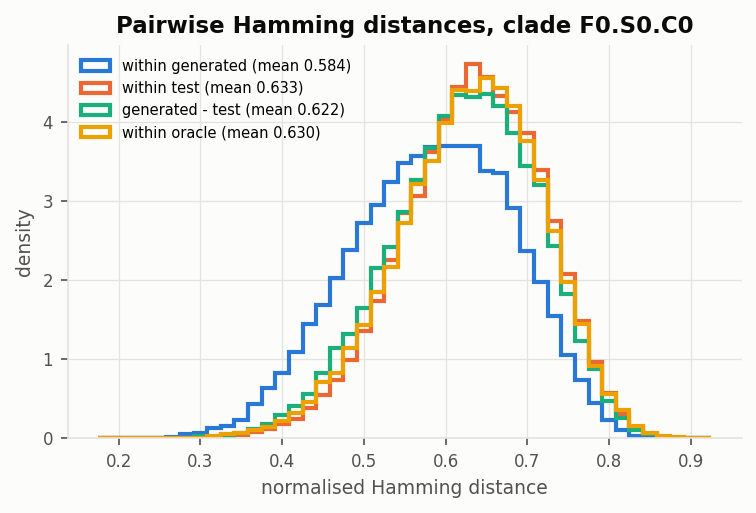
\includegraphics[width=0.49\linewidth]{models/fa_conditional_H128/dist_pairwise_F0.S0.C0.png}\hfill
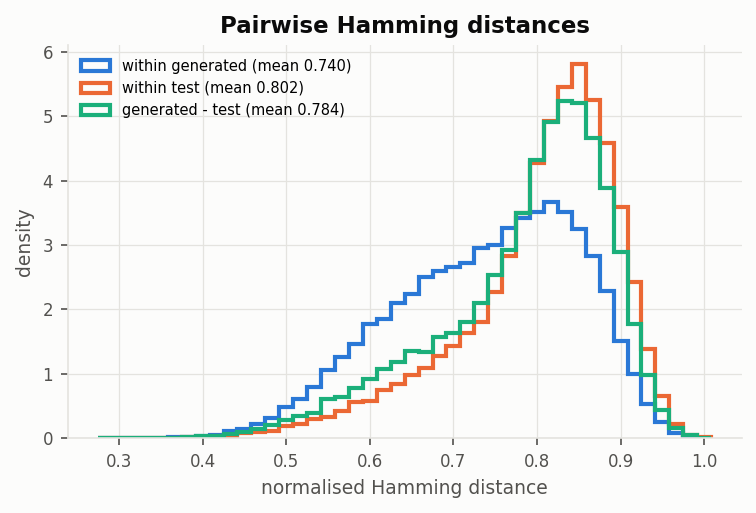
\includegraphics[width=0.49\linewidth]{models/fa_unconditional_H128/dist_pairwise.png}
\caption{Pairwise Hamming distance distributions. Left: clade \texttt{F0.S0.C0} with its tag (within generated, within
test, generated--test, within oracle). Right: unconditioned model, pooled over all clades.}
\end{figure}

\subsection{Position in PCA space: Fréchet distance}
The ladder built from the ground truth (\S\ref{sec:distances}), the Fréchet distance between the test sequences of
two clades, is
\begin{center}\small
\begin{tabular}{lcccc}
\toprule
 & same clade (oracle) & sibling clade & same family, other subfamily & other family\\
\midrule
FD (mean) & 0.02 & 1.48 & 6.15 & 21.4\\
\bottomrule
\end{tabular}
\end{center}
It spans three orders of magnitude, which makes it a sharp tool for placing a generated set in the hierarchy.
\begin{itemize}
\item \textbf{Conditioned $H=128$}: the generated clade vs its own test clade has FD $=0.39$ on average
(range 0.07--1.06). That is between the oracle (0.02) and the sibling clade (1.48). Even the worst generated clade (1.06) is closer
to its own test set than the average true sibling clade (1.48). For 17 of 18 generated clades the closest test clade
is their own (FD assignment accuracy 94\%; the $r_C$ assignment gave 18/18).
\item \textbf{Unconditioned $H=128$}, pooled: FD $=2.23$ against 0.001 for the oracle. The cloud is misplaced as a
whole because of the family weights.
\end{itemize}

\begin{figure}[H]
\centering
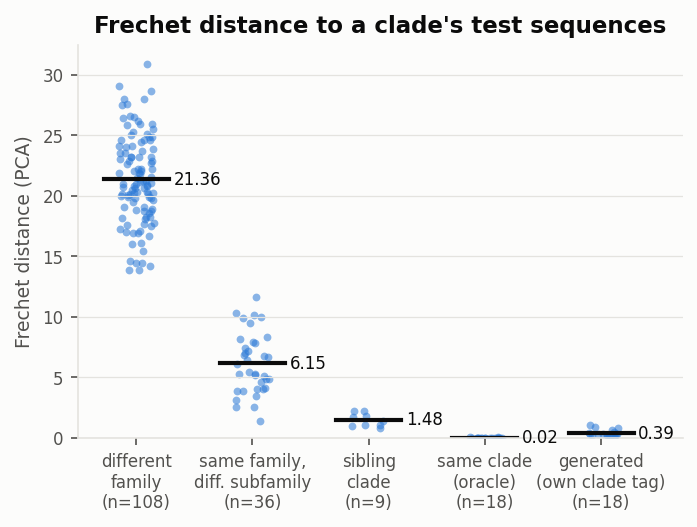
\includegraphics[width=0.49\linewidth]{models/fa_conditional_H128/frechet_ladder.png}\hfill
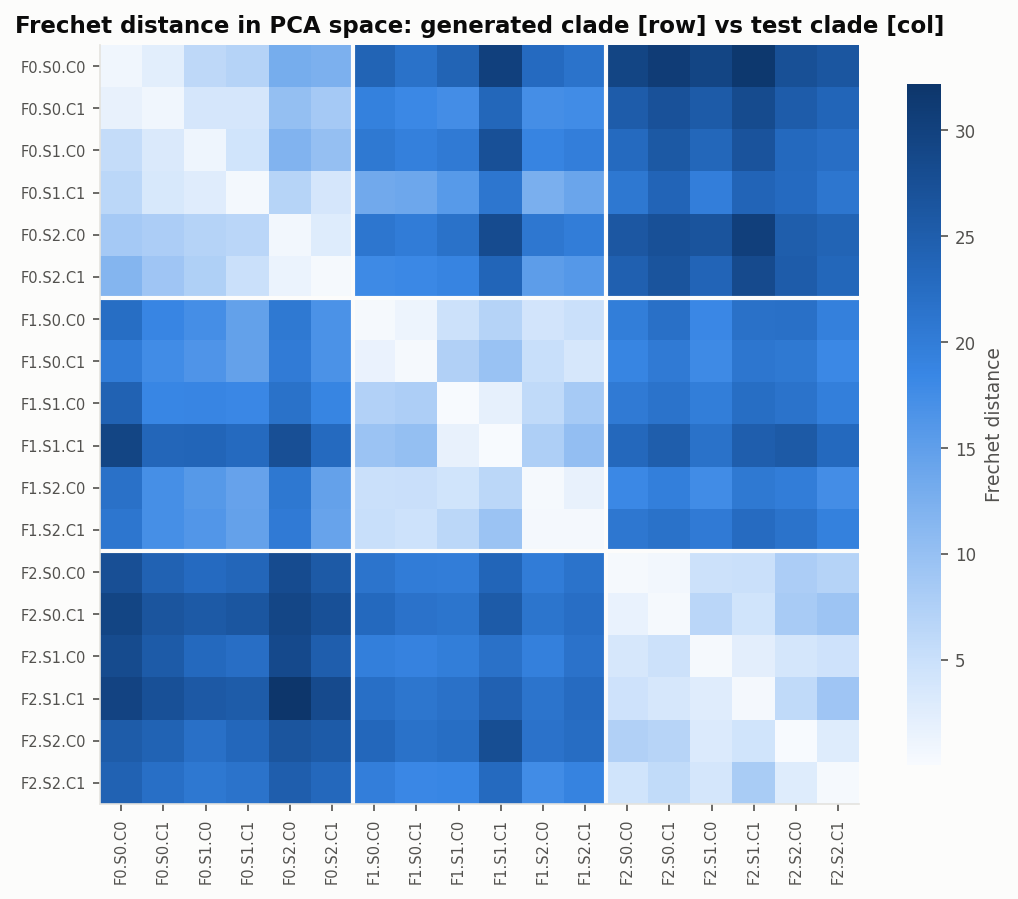
\includegraphics[width=0.49\linewidth]{models/fa_conditional_H128/cross_clade_frechet.png}
\caption{Left: FD to a clade's test sequences, for test sets of other clades grouped by relation (the ground-truth
ladder) and for the sequences generated with the clade's own tag (right-most column). Right: FD between each
generated clade (row) and each test clade (column); the dark diagonal and the family blocks are the hierarchy.}
\end{figure}

\begin{keybox}{What the distances add}
The three distance families agree with the statistics of \S\ref{sec:res_cond} and add two things:
(i) \textbf{no memorisation} (no copies, novelty equal to that of real held-out sequences); and
(ii) a \textbf{direct position in the hierarchy}: a generated clade is about 4 times closer to its own clade than
the sibling clade is (FD 0.39 vs 1.48), but 20 times farther than a perfect generator would be (0.02). Its
remaining defect is a small loss of diversity (1.6 sites), the sequence-level signature of fields that are too sharp.
\end{keybox}
